% ===========================================================
% methodology.tex
% ===========================================================
\section{Methodology}
\label{sec:methodology}

The pipeline is a directed acyclic graph of stages whose final two
nodes are the \texttt{cen2gtopt} canonical-feed builder
(\texttt{gtopt\_canonical\_feed}) and the marginal-unit identifier
(\texttt{gtopt\_marginal\_units}); every CEN/SCVIC/PLEXOS
extractor is wrapped by a hash-keyed parquet cache so that any
upstream change short-circuits at the first byte that has changed
(Fig.~\ref{fig:pipeline}).  Three operating modes are exposed:
\texttt{simulated} (re-solve a reduced LP), \texttt{real} (use the
published cleared dispatch), and \texttt{real-reconstruct} (the
default — the closest-CV picker over the SCVIC merit ladder); a
\texttt{compare} mode runs all three side-by-side for cross-checking.

\begin{figure}[t]
  \centering
  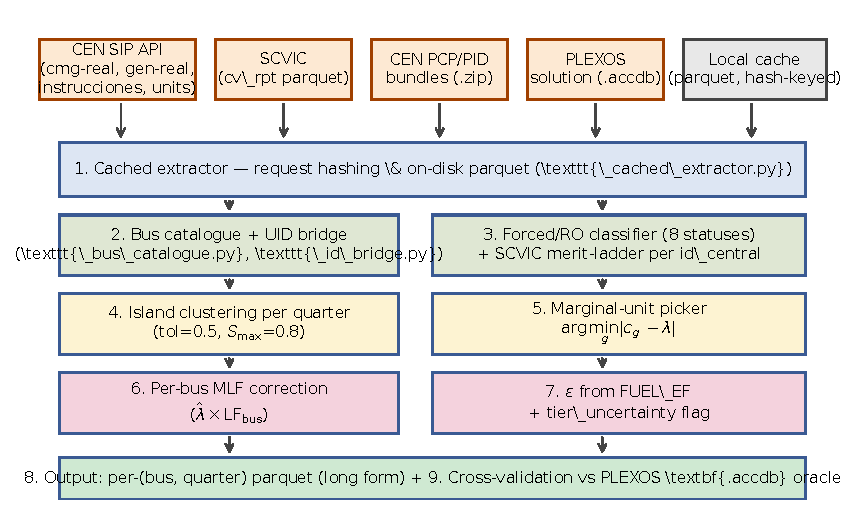
\includegraphics[width=\columnwidth]{figures/fig_pipeline_flow.pdf}
  \caption{The \texttt{cen2gtopt} pipeline with hash-keyed parquet
  caching at every CEN/SCVIC/PLEXOS extractor.
  \texttt{gtopt\_canonical\_feed} produces the per-block parquet feed
  consumed by \texttt{gtopt\_marginal\_units} in
  \texttt{real-reconstruct} mode (default).}
  \label{fig:pipeline}
\end{figure}

\subsection{Notation}
\label{sec:notation}

Time is partitioned into operating days, hours, and quarters
(\SI{15}{\minute} blocks).  $\setT=\{0,\ldots,95\}$ indexes
quarters; the network exposes a bus set $\setN$ at which CEN
publishes a nodal marginal cost $\lambda^{\mathrm{CEN}}_{b,t}$.
Each generator $g\in\setG$ has a fuel label $f(g)$, a technical
minimum $\underline{p}_g$, an effective maximum $\overline{p}_g$,
and a piecewise SCVIC ladder $\Phi_g=\{\phi\}$ of declared variable
costs $c_{g,\phi}$.  Per-hour realised dispatch is $p_{g,h}\in\R_+$.

The pipeline emits per (bus, quarter):
$\hat\lambda_{b,t}$ (reconstructed marginal price), $m_{b,t}\in\setG$
(marginal unit), $c_{m,\phi^\star}$ (its picked CV),
$\varepsilon_{m}$ (its fuel-default emission factor in
$\si{\tonne\mathrm{CO}_2\per\MWh}$), $\mathrm{LF}_{b,t}$ (bus loss
factor), and
$\varepsilon^{\mathrm{bus}}_{b,t}=\varepsilon_m\!\cdot\!\mathrm{LF}_{b,t}$.

\subsection{Inputs and bus catalogue}
\label{sec:inputs}

Table~\ref{tab:inputs} catalogues the CEN, SCVIC, and PLEXOS feeds
consumed by the pipeline.  All feeds are hash-keyed in the on-disk
parquet cache (\texttt{\_cached\_extractor.py}).  The CEN data
triplet uses three different bus identifiers (\texttt{id\_info},
17-character \texttt{bar\_transf}, and PLEXOS CamelCase node names);
\texttt{\_id\_bridge.py} reconciles them via Unicode-folding plus a
generator-of-aliases pass, with a hand-curated overrides table for
the residual cases.  The current catalogue contains \num{29}
reconciled \SI{220}{\kV}/\SI{500}{\kV} backbone buses; lower-voltage
buses share the nodal price of their backbone parent in CEN's PLEXOS
topology.

\begin{table}[t]
  \centering
  \caption{Public-data inventory consumed by \texttt{cen2gtopt}.
  Every feed is hash-keyed in the on-disk parquet cache; ``settled''
  is post-closeout, ``intra-day'' is the PID re-clear, ``day-ahead''
  is the PCP forecast.}
  \label{tab:inputs}
  % Public-data feed inventory table (Section 4.2)
\begin{tabularx}{\textwidth}{l l l l X}
  \toprule
  Feed & Service & Endpoint / file & Type & Notes \\
  \midrule
  cmg-real          & CEN SIP   & \texttt{/costo-marginal-real/v4/findByDate}     & settled    & 15-min nodal $\lambda$; 02:30 publication delay (10-quarter morning gap). \\
  cmg-online        & CEN SIP   & \texttt{/costo-marginal-online/v4/findByDate}   & intra-day  & 15-min nodal $\lambda$; full 24-h coverage; pre-validation, three version codes. \\
  generaci\'on-real & CEN SIP   & \texttt{/generacion-real/v3/findByDate}         & settled    & Hourly per-central dispatch in MW. \\
  instrucciones-cmg & CEN SIP   & \texttt{/instrucciones-operacionales-cmg/v4/findByDate} & settled & Per-hour state \texttt{estado} and consigna \texttt{CI/MT/PMT/PP/PS/PC}; price-taker classifier. \\
  unidades-generadoras & CEN SIP & \texttt{/unidades-generadoras/v4/findByDate}   & static     & Per-unit pmin, pmax, fuel, technology, alias names. \\
  generaci\'on-programada-pcp & CEN SIP & \texttt{/generacion-programada-pcp/v4} & day-ahead  & PCP-LP-output dispatch per central per hour. \\
  cmg-programado-pcp          & CEN SIP & \texttt{/cmg-programado-pcp/v4}         & day-ahead  & PCP-cleared $\lambda$ per bus per hour; implicit hydro water value. \\
  embalse-real      & CEN SIP   & \texttt{/embalse-real/v3}                       & settled    & Reservoir levels (cota msnm) per embalse per day. \\
  flujo-programado-pcp & CEN SIP & \texttt{/flujo-programado-pcp/v4}             & day-ahead  & Programmed line flows; useful for binding-line / island detection. \\
  limitaciones      & CEN SIP   & \texttt{/limitaciones-transmision/v4/findByDate} & settled & Line outages and operational restrictions per day. \\
  \midrule
  cv\_rpt           & SCVIC     & \texttt{cv\_rpt\_YYYY\_MM.parquet}              & static (monthly) & Piecewise CV declaration per generator per fuel per tier. \\
  \midrule
  PCP bundle        & PCP archive & \texttt{PCP\_YYYYMMDD.zip}                    & day-ahead  & PLEXOS XML inputs for the day-ahead clear. \\
  PCP solution      & PCP archive & \texttt{PCP\_RES\_YYYYMMDD/\dots\,Solution.accdb} & settled & PLEXOS solver-output per-bus $\lambda$, per-unit dispatch, per-bus MLF. \\
  PID bundle        & PID archive & \texttt{PID\_YYYYMMDD\_HH/\dots\,Solution.accdb} & intra-day & PLEXOS intra-day re-clear, settlement-binding. \\
  \bottomrule
\end{tabularx}

\end{table}

\subsection{Operational-state classification}
\label{sec:classifier}

Each generator at each hour falls into one of eight mutually
exclusive operational states (Table~\ref{tab:classifier}).
Price-taker units (those held at a technical minimum or
operator-imposed setpoint) cannot supply the next \SI{1}{\MWh} of
energy and so cannot set the marginal price.  The classifier reads
\texttt{instrucciones-operacionales-cmg} and flags as forced any
unit with \texttt{estado}$\ne$\texttt{N} or
\texttt{consigna}$\in$\{\texttt{CI}, \texttt{MT}, \texttt{PMT},
\texttt{PP}, \texttt{PS}, \texttt{PC}\}.  A subtle extension of the
classical PJM treatment: forced units \emph{at interior dispatch}
($\underline{p}_g+\delta<p_g<\overline{p}_g-\delta$ with
$\delta=0.05(\overline{p}_g-\underline{p}_g)$) remain valid
marginal-unit candidates because the next \SI{1}{\MWh} can come from
them.  Only forced-at-pmin units are excluded.

\begin{table}[t]
  \centering
  \caption{Operational-state classification.  Priority is evaluated
  top-down: the first matching row determines the unit's status.}
  \label{tab:classifier}
  % 8-status priority-ordered rule table (Section 4.4)
\begin{tabular}{rlll}
  \toprule
  \# & Status (regime) & Trigger condition & Treatment in picker \\
  \midrule
  1 & \texttt{demand\_fail}             & $\lambda^{\mathrm{CEN}}_{b,t} > \$800$/MWh                       & $\varepsilon{=}0$, marginal $=$ \texttt{demand\_fail\_cost} \\
  2 & \texttt{renewable\_curtailment}   & $\lambda^{\mathrm{CEN}}_{b,t} \le \$0.5$/MWh                     & $\varepsilon{=}0$, marginal $=$ \texttt{renewable\_curtailment} \\
  3 & \texttt{no\_candidates}           & no dispatched units in island                                    & propagate \texttt{NaN}; flag for analyst review \\
  4 & \texttt{no\_cv\_match}            & all dispatched have empty SCVIC ladder OR all forced-at-pmin    & propagate \texttt{NaN}; flag \\
  5 & forced-at-pmin (\textit{drop})    & \texttt{consigna}$\in\{$CI,MT,PMT,PP,PS,PC$\}$ AND $p_g \le \underline{p}_g + \delta$ & excluded from candidate pool \\
  6 & \texttt{matched\_capped\_pmax}    & picked $g$ with $p_g \ge \overline{p}_g - \delta$                & valid; energy must come from off-merit unit \\
  7 & \texttt{matched\_above}           & picked $g$ has $c_{g,\phi^\star} > \lambda$                      & valid; closest-CV is the next-up tier \\
  8 & \texttt{matched\_interior}        & picked $g$ has $\underline{p}_g + \delta < p_g < \overline{p}_g - \delta$ & valid; the canonical case \\
  \bottomrule
\end{tabular}
\\[3pt]
{\footnotesize Priority is evaluated top-down: the first matching
row determines the unit's regime at the (bus, quarter).
$\delta = 0.05(\overline{p}_g-\underline{p}_g)$ is the interior
tolerance.  Forced units at \emph{interior} dispatch remain valid
candidates: rule~5 only excludes the forced-at-pmin case.}

\end{table}

\subsection{Island clustering}
\label{sec:island}

Buses sharing a nodal marginal price in a given quarter are
electrically coherent in the merit-clearing sense.  Pure pairwise
$\lambda$-grouping exhibits a chained-clustering pathology: a
sequence such as
$(\$41.5,\$41.7,\$41.9,\$42.1,\$42.3,\$42.7)$ with
$\Delta_{\mathrm{tol}}=\$0.5$ collapses to a single island despite
the \$1.20 endpoint spread.  After sorting buses ascending by
$\lambda$, the pipeline starts a new island whenever
\begin{equation}
\lambda_b - \lambda_{b-1} > \Delta_{\mathrm{tol}}
\quad\lor\quad
\lambda_b - \lambda^{\mathrm{isl,min}} > S_{\max},
\label{eq:island}
\end{equation}
with $\Delta_{\mathrm{tol}}=\$0.5$/MWh and $S_{\max}=\$0.8$/MWh in
production.  Fig.~\ref{fig:island} contrasts the pure pairwise walk
with the cumulative-spread walk.

\begin{figure}[t]
  \centering
  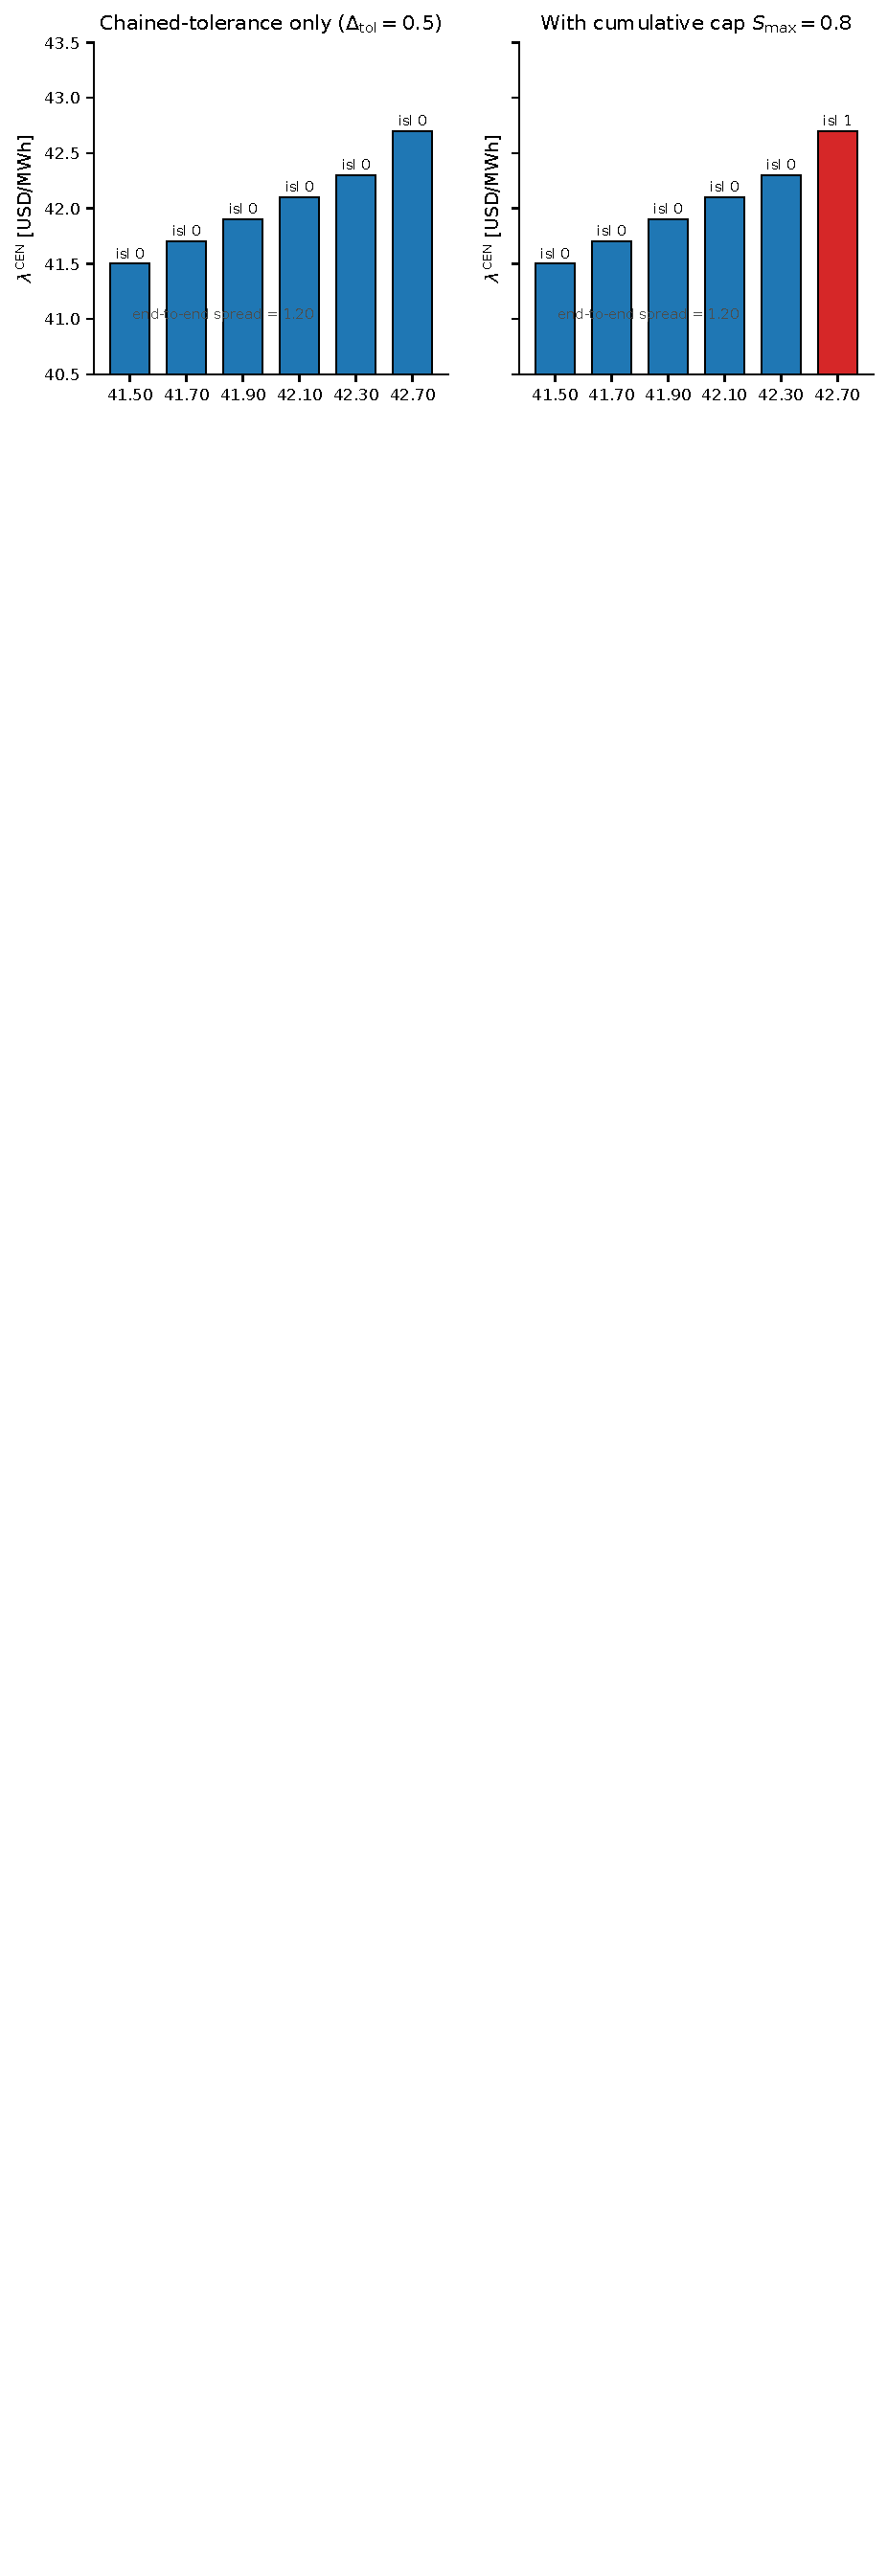
\includegraphics[width=\columnwidth]{figures/fig_island_clustering_demo.pdf}
  \caption{Island clustering with chained tolerance only
  (\textit{left}) vs.\ chained tolerance with cumulative-spread cap
  $S_{\max}=\$0.8$ (\textit{right}).}
  \label{fig:island}
\end{figure}

\subsection{Per-bus loss-factor correction}
\label{sec:mlf}

The reconstructed price is the product of the marginal-unit CV and
the bus loss factor:
\begin{equation}
\hat\lambda_{b,t} = c_{m_{b,t}, \phi^\star} \cdot \mathrm{LF}_{b,t}.
\label{eq:lambda-bus}
\end{equation}
The pipeline supports two estimators in priority order.  The
\emph{primary} estimator reads the PLEXOS-solver-output Marginal
Loss Factor from the PID solution \texttt{.accdb} for the day,
attached to \texttt{System.Nodes} at \texttt{collection\_id=281};
this is the exact value used at LP clearing, extracted by
\texttt{pcp\_solution.py} via \texttt{mdbtools}.  The \emph{fallback}
is a per-quarter empirical ratio
\begin{equation}
\mathrm{LF}^{\mathrm{emp}}_{b,t} =
  \frac{\lambda^{\mathrm{CEN}}_{b,t}}
       {\lambda^{\mathrm{CEN}}_{r,t}},
\label{eq:lf-emp}
\end{equation}
where the reference bus $r$ is the lowest-\texttt{id\_info} bus
present in the quarter.  When both are available the ratio
$\mathrm{LF}^{\mathrm{PID}}_{b,t} =
\mathrm{LF}^{\mathrm{bus}}/\mathrm{LF}^{\mathrm{unit}}$ cancels
generator-side losses.

\subsection{SCVIC merit ladder and PLEXOS PID overlay}
\label{sec:scvic}

Each generator declares to the Coordinador a piecewise variable
cost $c_{g,\phi}$ as a function of configuration (fuel, load tier,
ambient).  The pipeline filters tiers below a per-fuel CV floor
(\SI{30}{\USD\per\MWh} for GNL/GLP/gas-propano,
\SI{15}{\USD\per\MWh} otherwise) and tiers above
\SI{1000}{\USD\per\MWh} (PLEXOS sentinels).
Fig.~\ref{fig:ladder} illustrates a multi-tier GNL CCGT and a
coal-fired unit.

\begin{figure}[t]
  \centering
  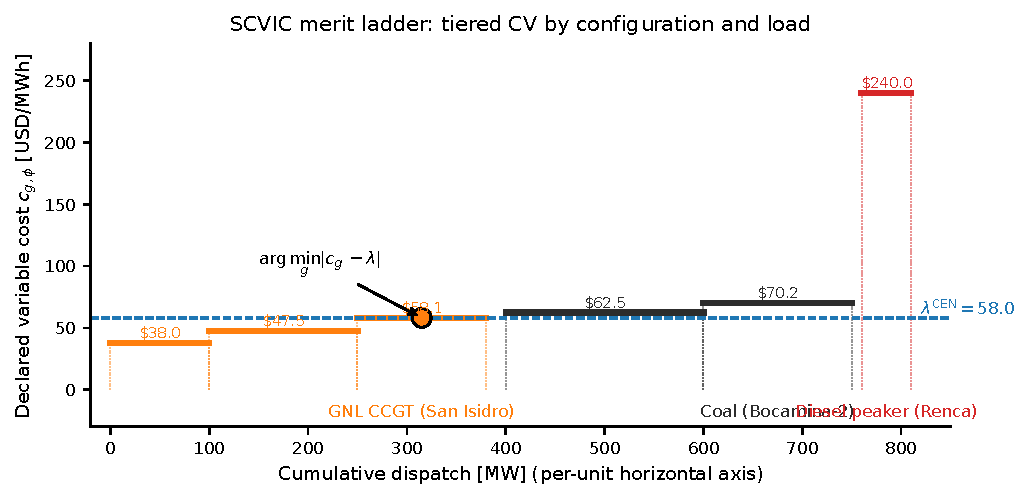
\includegraphics[width=\columnwidth]{figures/fig_scvic_ladder_example.pdf}
  \caption{SCVIC merit ladder for three illustrative units.  The
  picker selects the tier whose CV is closest in absolute value to
  the target $\lambda$; the highlighted marker shows the picked tier
  for $\lambda=\SI{58}{\USD\per\MWh}$.}
  \label{fig:ladder}
\end{figure}

\paragraph{PLEXOS PID overlay (v3 picker).}
SCVIC declares price tiers but not the binding technical-minimum
that the LP actually clears against.  The v3 picker overlays the
PLEXOS PID-extracted $\underline{p}_g$ and $\overline{p}_g$ from the
\texttt{.accdb} on top of the SCVIC ladder, taking the maximum of
the three declared MTs (master-table) values as the binding
$\underline{p}_g$.  This eliminates ``forced-at-pmin'' false
negatives in the candidate pool that arise when the SCVIC-declared
$\underline{p}_g$ is lower than the operator-imposed value.  The
overlay is opt-in to preserve compatibility with cases where the
PID archive is unavailable.

\subsection{Marginal-unit identification}
\label{sec:identify}

The picker (Algorithm~\ref{alg:identify}) treats the candidate pool
as the dispatched non-forced (or forced-but-interior) units with at
least one SCVIC tier and selects the unit whose nearest tier
minimises $|c_{g,\phi}-\lambda|$.  The returned record carries a
regime label drawn from \texttt{matched\_interior},
\texttt{matched\_capped\_pmax}, \texttt{matched\_near\_pmin},
\texttt{matched\_above}, \texttt{no\_candidates},
\texttt{no\_cv\_match}, \texttt{renewable\_curtailment}, or
\texttt{demand\_fail}; these labels propagate to the output parquet
and the per-day diagnostic report.

\begin{algorithm}[t]
\caption{Marginal-unit identification per island}
\label{alg:identify}
\begin{algorithmic}[1]
  \REQUIRE $\lambda_{\mathrm{tgt}}$, candidate set $\setC$, ladders
           $\{\Phi_g\}$, fuel labels $\{f(g)\}$, forced flag
           $F_g\in\{0,1\}$
  \IF{$\lambda_{\mathrm{tgt}}\le\$0.5$}
    \STATE \RETURN regime $=$ \texttt{renewable\_curtailment},
           $\varepsilon=0$
  \ELSIF{$\lambda_{\mathrm{tgt}}>\$800$}
    \STATE \RETURN regime $=$ \texttt{demand\_fail},
           $\varepsilon=0$
  \ENDIF
  \STATE pool $\leftarrow \{g\in\setC : \Phi_g \ne \emptyset\}$
  \STATE annotate each $g$ via $\delta=0.05(\overline{p}_g-\underline{p}_g)$
  \STATE drop $\{g : F_g=1 \land \mathrm{status}=\texttt{near\_pmin}\}$
  \IF{pool empty}
    \STATE \RETURN regime $=$ \texttt{no\_cv\_match}
  \ENDIF
  \FOR{$g\in\mathrm{pool}$}
    \STATE $c_g \leftarrow$ tier in $\Phi_g$ closest to
           $\lambda_{\mathrm{tgt}}$
  \ENDFOR
  \STATE $m \leftarrow \arg\min_{g\in\mathrm{pool}}
           |c_g - \lambda_{\mathrm{tgt}}|$
  \STATE \RETURN $m$, $c_m$, $f(m)$, regime
\end{algorithmic}
\end{algorithm}

\paragraph{LP-duality justification.}
The picker is the empirical realisation of the merit-order
identity $\lambda_t^\star = c_{m(t)}$ for any generator $m(t)$
strictly interior to its bounds in the cost-minimising dispatch.
Replacing the cost coefficient $c_g$ by an emission coefficient
$e_g$ leaves the constraint structure intact and produces the
emission-marginal value $\varepsilon_t^\star = e_{m'(t)}$ at the
optimum.  The pipeline relies on the assumption $m(t)=m'(t)$ — that
the cost-marginal and emission-marginal units coincide — which holds
whenever the picked unit is the unique strictly-interior generator
at block $t$.  Two pathologies break the assumption: degenerate cost
ties between fuels with distinct $e_g$, and forced-interior units
(by construction excluded).  Both are flagged in
\texttt{tier\_uncertainty} and surface in the audit oracle.  A
joint primal $\min_p\sum_g(c_g+p_{\mathrm{CO}_2}e_g)p_g$ reads off
the gas-vs-coal switching price
$p^\star=(c_2-c_1)/(e_1-e_2)\!\approx\!\SI{56}{\USD\per\tonne CO_2}$
for the representative Chilean coal-vs-gas pair, squarely inside the
EU~ETS~2025 trading range.

\subsection{Marginal emission factor}
\label{sec:eps}

The fuel-default emission table $\varepsilon_f$
(Table~\ref{tab:fuelef}) is derived from IPCC~2006~GL Vol.~2 Tab.~1.4
multiplied by typical SEN heat rates.  The bus-level marginal
emission factor is
\begin{equation}
\varepsilon^{\mathrm{bus}}_{b,t} = \varepsilon_{f(m_{b,t})}
                                   \cdot \mathrm{LF}_{b,t},
\label{eq:eps-bus}
\end{equation}
and the embedded carbon-tax cost is
$\tau_{\mathrm{CO}_2}\varepsilon^{\mathrm{bus}}_{b,t}/1000$ in
\si{\USD\per\MWh} with $\tau_{\mathrm{CO}_2}=\SI{5}{\USD\per\tonne CO_2}$
under Law~20.780.

\begin{table}[t]
  \centering
  \caption{Fuel-default emission factors $\varepsilon_f$
  (\si{\kg\mathrm{CO}_2\per\MWh}).  IPCC 2006 GL Vol.~2 Tab.~1.4 ×
  typical SEN heat rates; biomass and biogas are biogenic-zero.}
  \label{tab:fuelef}
  % Fuel emission factor table (Section 4.9)
\begin{tabular}{l r l}
  \toprule
  Fuel (SCVIC label)        & $\varepsilon_f$ [kg CO$_2$/MWh] & Provenance \\
  \midrule
  Carb\'on / Carb\'on + Petcoke / Petcoke & 1062 & IPCC 2006 GL Vol.~2, hard coal × \SI{2.45}{\GJ\per\MWh} \\
  Diesel / Di\'esel / Petr\'oleo Di\'esel &  847 & IPCC 2006 GL, distillate fuel oil \\
  Fuel Oil / Fuel Oil Nro.~6              &  780 & IPCC 2006 GL, residual fuel oil \\
  Gas Natural / GNL                       &  380 & IPCC 2006 GL, natural gas × CCGT efficiency \\
  GLP / Gas Propano                       &  700 & IPCC 2006 GL, LPG \\
  Cogeneraci\'on                          &  400 & Mixed: assumed half-natural-gas, half-biogenic \\
  Biomasa / Biogas                        &    0 & IPCC biogenic-zero (Tier~1) \\
  Geot\'ermica                            &    0 & non-fossil (CO$_2$-fugitive emissions $<$ 1\%) \\
  Hidr\'aulica / Solar / E\'olica         &    0 & non-emitting renewable \\
  \bottomrule
\end{tabular}
\\[3pt]
{\footnotesize Emission factors are quoted per \si{\MWh} of
electrical output, embedding a typical SEN heat-rate assumption
per fuel.  Units are kg\,CO$_2$/MWh; division by 1000 yields
\si{\tonne\mathrm{CO}_2\per\MWh}.  Mixed cogeneration reflects
the dominant fuel mix at SEN cogeneration plants
(half natural gas, half biogenic woodchip).}

\end{table}

A per-cell \texttt{tier\_uncertainty} flag is set when the picked
tier is more than \$2/MWh below the next-up CV in the same unit's
ladder; \SI{13.7}{\percent} of cells are wedge-flagged on
2026-04-22.  Downstream consumers can treat $\hat\lambda$ as a lower
bound on these cells.

\subsection{Cross-validation against the PLEXOS oracle}
\label{sec:oracle}

The PCP/PID solution \texttt{.accdb} is parsed by
\texttt{pcp\_solution.py}, exposing per-period system shadow prices,
per-unit dispatch, and per-bus MLFs.  Three quantities are read for
cross-validation: per-bus $\lambda$ (compared against
$\lambda^{\mathrm{CEN}}$ to validate the publication chain), per-unit
dispatch $p_{g,h}^{\mathrm{PLEXOS}}$ (compared against SIP
\texttt{generaci\'on-real}), and the per-bus MLF.  When both PCP and
PID bundles are on disk, PID values take precedence — the intra-day
re-clear is the binding settlement reference.  The oracle also yields
the post-hoc $\hat\lambda^{\mathrm{PID}}_{b,t}$ column in the output
parquet, computed using $\mathrm{LF}^{\mathrm{PID}}_{b,t}$ in
\eqref{eq:lambda-bus}.
